\section{OPQ Mauka}
\label{sec:opq-mauka}

The previous sections discussed the design of OPQ Box, a custom hardware device for collecting four important measures of power quality, and OPQ Makai, a novel, hybrid centralized/decentralized data acquisition scheme which involves two-way communication between the OPQ Boxes.  As a result of these two innovations, an OPQ sensor network has the ability to collect and analyze high fidelity, low level data about power quality anomalies in a cost-effective, scalable fashion.

There are remaining challenges to creating a useful power quality sensor network. First, the data provided by OPQ Boxes is low-level, "primitive" data consisting of either features (i.e. frequency, voltage, THD, and transients) or waveform data. But what we actually want is actionable insights into grid stability. For example, we might want to know if a given anomalous data value is actually detrimental, or we might want to be able to predict when a power quality event might occur in the future based upon the recognition of cyclical events in the historical data.

A second challenge involves the potentially high volume of data might accumulate in the cloud. Although OPQ Box and OPQ Makai provide a scalable mechanism for communicating power quality data to the cloud services, it is still the case that, over time, a substantial amount of data could accumulate. One strategy is to simply store all of the data sent to the cloud forever. This means that data storage requirements will increase monotonically over time, making the sensor network more costly to maintain the longer it is in place. An alternative strategy is to implement an algorithm to identify uninteresting (or no longer interesting) data and discard it.  Ideally, such an algorithm would enable OPQ sensor network designers to calculate an upper bound on the total amount of cloud storage required as a function of the number of nodes (OPQ Boxes) in the network.

OPQ Mauka addresses both of these issues. First, OPQ Mauka provides a multi-layered representation for structuring and processing DSN data. The structure and processing at each layer is designed with the explicit goal of turning low-level data into actionable insights. Second, each layer in the framework implements a "time-to-live" (TTL) strategy for data within the level. This strategy states that data must either progress upwards through the layers towards more abstract, useful representations within a fixed time window, or else it can be discarded. The TTL strategy is useful because when implemented, it allows DSN designers to make reasonable predictions of the upper bounds on data storage at each level of the framework.

 TTL also makes possible a "graceful degradation" of system performance if those bounds turn out to be exceeded. For example, consider a situation in which a power network enters a prolonged period of widespread power quality instability, where every OPQ Box is reporting continuous anomalous conditions with respect to voltage, frequency, THD, and transients.  This "worst case scenario" would lead to the potential situation of every OPQ Box trying to upload raw waveform data all the time. The TTL system provides safeguards, in that whatever low-level data has not been processed relatively quickly can be discarded.  Thus, instead of the system potentially going down entirely, it could instead continue to operate at a reduced capacity.

Figure \ref{fig:mauka-data-model} illustrates the hierarchical data model for OPQ Mauka. This data model can be conceptualized as a multi-level hierarchy that adaptively optimizes data storage using a tiered TTL approach and provides a mechanism in which typed aggregated data is continually refined to the point of being of becoming actionable. The data model also includes software components called "actors" that both move data upward through the levels and apply optimizations downward through the levels. Actors are implemented through a plugin architecture, making it easy to experiment with the data model and improve it over time.

\begin{figure}
\center 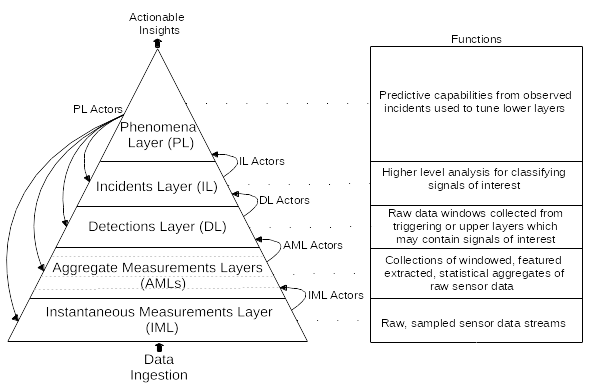
\includegraphics[width=4in]{images/mauka/mauka-data-model.png}
\caption{Mauka data model hierarchy}
\label{fig:mauka-data-model}
\end{figure}

The lowest layer of the hierarchy is the Instantaneous Measurements Layer (IML). The IML contains "raw" data, in other words, the digitize waveform.  IML data exists both on each OPQ Box (where it is available for up to the previous 60 minutes). It also exists in the cloud, in the event that OPQ's triggering mechanism has caused a temporal interval of waveform data to be uploaded. IML data in the cloud has a TTL of 15 minutes: unless the wave form data is found to be useful by a cloud service within 15 minutes, it can be discarded.

The second layer is the Aggregate Measurements Level (AML). The AML stores power quality summary statistics sent either once per second or once per minute by each OPQ Box. These summary statistics include the maximum, minimum, and average values of voltage, frequency, and THD over the time window, as well as the presence or absence of transients. It is AML data that is used to initiate the triggering process of uploading IML data from the cloud.

The third layer is the Detections Level (DL). This layer is responsible for processing the IML and AML data to produce a representation of an "event" with a precisely defined start and end time based upon examination of the waveform.  As will be discussed in Section \ref{sec:subthreshold-events}, knowledge of the start and end time of a power quality anomaly allows investigation of how that anomaly might manifest itself elsewhere in the grid, even if this manifestation is not severe enough to produce over-threshold data values.

The fourth layer is the Incident Level (IL).  This layer starts to answer the question of whether or not the data is "actionable" by classifying the detected event according to various industry standards for power quality anomalies: IEEE 1159, ITIC, SEMI F47, and so forth.  For example, an event that falls into the ITIC "prohibited" region clearly indicates a power quality anomaly that requires further study and intervention.

The fifth and final level is the Phenomena Layer (PL). This layer contains the results of analyses that attempt to identify cyclic, and thus predictable, power quality disturbances. It also contains analysis results regarding the similarity of various incidents, which can help uncover causal factors.  Finally, it provides analyses for adaptive optimization of the OPQ Sensor Network. These optimizations can change the thresholds for individual boxes to either increase their sensitivity or decrease their sensitivity over specific intervals of time. The ultimate goal of adaptive optimization is to help the network learn to acquire all of the data useful for analyses, and only the data useful for analyses.  We are still in the early stages of exploring the potential of adaptive optimization in OPQ networks.

\subsection{OPQ Mauka Actors}

The current capabilities of OPQ Mauka can be summarized in terms of its Actors, which are implemented as plugins. Nine of the most important Actors are described below.

{\em Makai Event Actor.} The Makai Event Actor is responsible for reading data newly created by OPQ Makai into OPQ Mauka. It performs feature extraction on the raw data stream and forwards those features (or the raw data) to subscribing Actor plugins. This allows OPQ Mauka to perform feature extraction once, and allow use of those features by multiple Actors.

{\em Frequency Variation Actor.} The Frequency Variation Actor classifies generic frequency sags, swells, and interruptions as defined by the IEEE 1159 standard. Both duration and deviation from nominal are used to perform these classifications. Duration classifications include frequency deviations that last for less than 50 ns, between 50 ns to 1 ms, and 1 ms to 50 ms. Classifications for deviations from nominal are performed for values that are up to 40\% deviation from nominal. This Actor is able to classify frequency swells, frequency interruptions, and frequency sags, leading to the creation of data at the Incident Layer.

{\em IEEE 1159 Voltage Actor.} The IEEE 1159 Voltage Actor is used to classify voltage Incidents in accordance with the IEEE 1159 standard[29]. In general, this standard classifies voltage disturbances by duration and by magnitude. Voltage durations are classified from 0.5 to 30 cycles, 30 cycles to 3 seconds, 3 seconds to a minute, and greater than 1 minute. Voltage deviations are classified in both the sag and swell directions as a percentage from nominal. Sags are generally classified between 10\% and 90\% of nominal while swells are generally classified from 110\% to 180\% of nominal. This Actor is capable of classifying voltage sags, swells, and interruptions as defined by the standard, and creating data at the Incident Layer if appropriate.

{\em Box Optimization Actor.} The Box Optimization Actor is responsible for sending and receiving typed messages to and from OPQ Boxes from OPQ Mauka. This Actor is capable of requesting the state of each OPQ Box (e.g. uptime, Measurement rate, security keys, etc). It is also capable of adjusting the state of individual OPQ Boxes by changing things such as the Measurement and Trend rate or the sampling rate used by the Box.

{\em Future Phenomena Actor.} The Future Phenomena Actor is responsible for creating Future or Predictive Phenomena. These Phenomena are used to predict Events and Incidents that may occur in the future. This plugin does not subscribe to any messages, but instead utilizes timers to perform its work. By default, this plugin runs every 10 minutes.

When a Future Phenomena Actor runs, it loads any active Periodic Phenomena found in the database. If Periodic Phenomena are found, this Actor extrapolates possible Detection and Incident Layer data by first examining their timestamps and then extrapolating into the future using the mean period and the standard deviation. For each timestamp in a Periodic Phenomena, the mean period is added. If the resulting timestamp is in the future, a Future Phenomena is created using the time range of the future timestamp plus or minus the standard deviation of the Periodic Phenomena.

When a Future Phenomena is created, timers are started in a separate thread signifying the start and end timestamps of the Future Phenomena. When the first timer runs, messages are sent to the Box Optimization Actor and the Threshold Optimization Actor instructing OPQ Box thresholds to be set lower and measurement rates to be set higher. This increases the chance of seeing an anomaly over the predicted time window. When the second timer runs, these values are reset to their default values. Thus, the plugin increases fidelity and decreases thresholds over the period of a Future Phenomena.

{\em ITIC Actor.} The ITIC Actor analyzes voltage to determine where it falls within the ITIC curve \cite{thallam_power_2000}. The ITIC curve is a power acceptability curve that plots time on the x-axis and voltage on the y-axis.  The purpose of the curve is to provide a tolerance envelope for single-phase 120V equipment. The curve defines three regions. The first region is "No Interruption" and generally includes all voltages with very short sustained durations. All events within this region have no noticeable effect on power equipment. The second region, the "No Damage Region", occurs during voltage sags for extended periods of time. Power Events in this region may cause equipment interruptions, but it will not damage the equipment. The final region, the "Prohibited" region, is caused by sustained voltage swells and may cause damage to power equipment. This Actor determines if an event falls within the "No Damage" or "Prohibited" regions and if so, creates an Incident to record this.

{\em SEMI F47 Actor.} The SEMI F47 Actor is similar to the ITIC Actor in that it plots voltage and duration against a power acceptability curve. In this case, the standard used is the SEMI F47 standard \cite{djokic_sensitivity_2005}. Rather than using a point-in-polygon approach, this plugin reads the voltage features sequentially and uses a state machine to keep track of the current classification. This plugin only classifies values as a "violation" or as "nominal".

{\em Transient Actor.} The Transient Actor is responsible for classifying frequency transients in power waveforms. The plugin subscribes to messages from a topic which contains a calibrated power waveform payload. The Transient Actor is capable of classifying impulsive, arcing, oscillatory, and periodic notching transients. A decision tree is utilized to select the most likely transient type and then further analysis is used to perform the actual classification of transients. Dickens et al \cite{dickens_transient_2019} provides more details on the transient classification system used by this Actor.

{\em Periodicity Actor.} The Periodicity Actor is responsible for detecting periodic signals in power data. This Actor does not subscribe to any messages, but instead runs off of a configurable timer. The Actor is set to run by default once an hour and every hour it scrapes the last 24 hours worth of data and attempts to find periods in the Measurements over that duration.

For each feature in the Measurement and Trend data (e.g. frequency, voltage, and THD), the Periodicity Actor first removes the DC offset from the data by subtracting the mean. Next, the Actor filters the signal using a 4th order high-pass filter to filter out noise. The Actor then performs autocorrelation on the signal followed by finding the peaks of the autocorrelation. The mean distance between the peaks of the autocorrelation provides the period of the signal.

The Periodicity Actor only classifies data as periodic if at least 3 peaks were found and the standard deviation of the period is less than 600 seconds (10 minutes). Once a positive identification has been made, peak detection is performed on the original signal. Once the plugin has the timestamps and deviations from nominal of the periodic signal of interest, the plugin can group Measurements, Trends, Detection Layer Events, and Incidents that were created during the periodic signals together as part of the Periodic Phenomena.



